\section{Word-Level Abstraction using Gr\"obner basis}
\label{sec:theory}
We are given a circuit $C$ with $k$-bit inputs and outputs that
performs a polynomial computation $Y = \F(A)$ over $\Fq = \Fkk$. Let
$P(x)$ be the {\it given} irreducible or primitive polynomial used for
field construction, and let $\alpha$ be its root, i.e. $P(\alpha) = 0
$. Note that we do not know the polynomial representation
$\F(A)$ and our objective is to identify (the coefficients of)
$\F(A)$. Let $\{a_0, \dots, a_{k-1}\}$ denote the primary inputs and
let $\{y_0, \dots, y_{k-1}\}$ be the primary outputs of $C$. Then, the
word-level and bit-level correspondences are: 
\begin{equation}
\label{eqn:words}
 A = a_0 + a_1 \alpha + \dots + a_{k-1} \alpha^{k-1}; ~~ Y = y_0 +
y_1 \alpha + \dots + y_{k-1} \alpha^{k-1};
\end{equation}

We analyze the circuit and model all the gate-level Boolean operators
as polynomials in ${\mathbb{F}}_2 \subset \Fkk$. To this set of
Boolean polynomials, we append the polynomials of Eqn
(\ref{eqn:words}) that relate the word-level and bit-level
variables. We model this set of polynomials as $F = \{f_1, \dots,
f_s\}$ over the ring $R = \Fq[x_1, \dots, x_d, Y, A]$. Here $x_1,
\dots, x_d$ denote, collectively, all the bit-level variables of the
circuit --- i.e. primary inputs, primary outputs and the intermediate
circuit variables --- and $Y, A$ the word-level variables. Denote the
generated ideal as $J = \langle F \rangle \subset R$. Also, let us
denote the (unknown) ``specification'' of the circuit as a polynomial 
$Y - \F(A)$; or equivalently as $Y + \F(A)$ and -1 = +1 over $\Fkk$.

As $Y = \F(A)$, clearly $Y + \F(A)$ {\it  agrees with the solutions}
to the circuit equations $f_1 = \dots = f_s = 0$. In computer 
algebra terminology, this means that $Y + \F(A)$ {\it vanishes on the
  variety}  $V_{\Fq}(J)$. If $Y + \F(A)$ vanishes on $V_{\Fq}(J)$,
then due to Proposition \ref{prop:finIV}, $Y + \F(A)$ is a member of
the ideal $I(V_{\Fq}(J))$. Strong Nullstellensatz over Galois fields
(Theorem \ref{thm:strong-nullsatz-fq}) tells us that $I(V_{\Fq}(J)) =
J + J_0$, where $J_0 = \langle x_1^q - x_1, \dots, x_d^q - x_d, Y^q -
Y, A^q - A \rangle$ is the ideal of vanishing polynomials in
$R$. Consolidating these results, we deduce that:

\begin{Proposition} 
\label{prop:spec_in_IV}
The specification polynomial $Y + \F(A) \in
  (J+J_0)$. 
\end{Proposition}

If the specification polynomial is known, then the verification
problem can be solved via membership testing of $Y + \F(A)$ in the
ideal $(J + J_0)$ (\cite{lv:date2012} actually used such a verification
formulation). We will now show further that by computing a Gr\"obner
basis of $(J + J_0)$, using a specific elimination term order, we can
also identify the polynomial $Y + \F(A)$ which represents the function
implemented by the circuit. 


{\bf Reverse-Engineering $\F$ from $C$:} The variety $V_{\Fq}(J)$ is
the set of all consistent assignments to the nets (signals) in the
circuit $C$. If we {\it project this variety on the word-level input and
output variables of the circuit $C$, we essentially generate the
function $f$ implemented by the circuit.} Projection of varieties from
$d$-dimensional space $\Fq^d$ onto a lower dimensional subspace
$\Fq^{d-l}$ is equivalent to {\it eliminating $l$ variables} from the
corresponding ideal. 

\begin{Definition}
    ({\bf Elimination Ideal}) From \cite{ideals:book}:  Given
  $J=\langle f_1,\dots,f_s\rangle \subset \Fq[x_1,\dots,x_d]$, the
  $l$th {\bf elimination ideal} $J_l$ is the ideal of
  $\Fq[x_{l+1},\dots,x_d]$ defined by 
    \begin{equation}
        J_l= J \cap \Fq[x_{l+1},\dots,x_d]
    \end{equation}
\end{Definition}

In other words, the $l$th elimination ideal does not contain variables
$x_1,\dots,x_l$, nor do the generators of it.  This can aid in solving
systems of polynomial equations by isolating variables in a set of
constraints, as is the purpose of techniques such as Gaussian
elimination. 
%The generators of a $k$th elimination ideal are such that
%$variables  are not present.
Moreover, Gr\"obner bases may be used to generate an elimination ideal
by using an ``elimination term order.''  One such ordering
is a pure lexicographic ordering, which features into a theorem:
%The ideal $I_k$ is spanned by elements which eliminate variables
%$x_1,\dots,x_k$.  This leads to an {\bf elimination theorem} for \Grobner
%bases:
\begin{Theorem} \label{thm:elim}
({\bf Elimination Theorem}) From \cite{ideals:book}: Let $J
  \subset \Fq[x_1,\dots,x_d]$ be an     ideal and let $G$ be a
  Gr\"obner basis of $J$ with respect to a lex ordering where $x_1
  > x_2 > \dots > x_d$.  Then for every $0     \leq l \leq
  d$, the set 
    \begin{equation}
        G_l= G \cap \Fq[x_{l+1},\dots,x_d]
    \end{equation}
    is a Gr\"obner basis of the $l$th elimination ideal $J_l$.
\end{Theorem}

We describe the application of elimination ideals using the following
example, borrowed from \cite{ideals:book}.

\begin{Example}

{\it 
Consider polynomials $f_1: x^2 - y - z - 1, ~~f_2: x - y^2 - z -1, 
~~f_3: x - y - z^2 - 1$ and ideal $J = \langle f_1, f_2, f_3\rangle
\subset {\mathbb{C}}[x, y, z]$. Let us compute a Gr\"obner basis $G$
of $J$ w.r.t. lex term order with $x > y > z$. Then $G = \{g_1, \dots,
g_4\}$ is obtained as: $g_1: x - y - z^2 - 1; ~~g_2: y^2 - y - z^2 - z;
~~g_3: 2yz^2 - z^4 - z^2; ~~g_4: z^6 - 4z^4 - 4z^3 - z^2$. 
Notice that the polynomial $g_4$ contains only the variable $z$, and
it {\bf eliminates} variables $x, y$. Similarly, polynomials $g_2,
g_3, g_4$, contain variables $y, z$ and eliminate $x$. According to
Theorem \ref{thm:elim}, $G_1 = G \cap {\mathbb{C}}[y, z] = \{g_2, g_3,
g_4\}$ and $G_2 = G \cap {\mathbb{C}}[z] = \{g_4\}$ are the Gr\"obner
bases of the $1^{st}$ and $2^{nd}$ elimination ideals of $J$, respectively.
}
\end{Example}

In conclusion, Gr\"obner basis computations w.r.t. pure lexicographic
term orders can be used to eliminate variables from an ideal. The
above example motivates our approach: Since we want to derive a
polynomial representation from a circuit in variables $Y, A$, we can
compute a Gr\"obner basis of $J + J_0$ w.r.t. an elimination order
that eliminates all the ($d$) bit-level variables of the
circuit. Then, the Gr\"obner basis $G_d = G \cap \Fq[Y, A]$ 
of the $d^{th}$ elimination ideal of $(J + J_0)$ will contain
polynomials in only $Y, A$. We now prove that the 
required polynomial representation will be found in $G_d$.
%$Y = \F(A)$
%will be found in $G_d$ and it will be the polynomial representation of
%the function implemented by the circuit.
First, let us formally ``setup'' the abstraction problem:

\begin{Setup}\label{not:abs}
Given a circuit $C$ with $k$-bit inputs and outputs which computes a
polyfunction $\F: \Fkk \rightarrow \Fkk$. Let $\{a_0, \dots, a_{k-1}\}$
be the bit-level primary inputs and $\{y_0, \dots, y_{k-1}\}$ be the
primary outputs. Let $A, Y$ denote the word-level input and output
variables of the circuit, respectively, such that $A = a_0 + a_1
\alpha + \dots + a_{k-1}\alpha^{k-1}$ and $Y = y_0 + \dots +
y_{k-1}\alpha^{k-1}$, where $\alpha$ is a primitive element of $\Fkk$. 
Let ${\mathcal{F}}(A)$ be the (unknown) polynomial representation of
the function implemented by the circuit such that $Y =
{\mathcal{F}}(A)$.  

Denote by $x_i, i = 1, \dots, d$ all the Boolean variables of the
circuit -- i.e. the input, output and the intermediate
variables. Let $R = \Fkk[x_i, Y, A: i = 1, \dots d]$ denote the
ring to model the polynomials that describe 
the circuit functionality. Let ideal $J \subset \Fkk[x_i, Y, A: i = 1
  \dots d]$ be generated by the bit-level and word-level polynomials
of the circuit. Let $J_0 = \langle x_i^2-x_i, Y^{2^k} - Y, A^{2^k} - A: i =
1, \dots, d\rangle$ denote the ideal of vanishing polynomials in $R$. 
\hfill$\Box$
\end{Setup}

Now, we will impose the following elimination order used for
abstraction: 

\begin{Definition}
{\bf Abstraction Term Order $>$:} 
%For the given circuit $C$,
%let $x_1, \dots, x_d$ denote all the bit-level variables, and let $Y,
%A$ denote, respectively the word-level output and input
%variables. 
Using the variable order $x_1 > x_2 > \dots > x_d > Y > A$,
impose a lex term order $>$ on the polynomial ring $R = \Fq[x_1,
  \dots, x_d, Y, A]$. This elimination term order $>$ is defined as
the {\bf Abstraction Term Order}. The relative ordering among $x_1,
\dots, x_d$ is not important and can be chosen arbitrarily. 
\end{Definition}


\begin{Theorem} \label{thm:abs}
{\bf Abstraction Theorem:} Using the setup and notations from {\it
  Problem Setup} \ref{not:abs} above, compute a Gr\"obner basis $G$ of
ideal $(J + J_0)$ using the abstraction term order $>$. Then: \\
(i) $G$ must contain the vanishing polynomial $A^q - A$ as the only
polynomial with only $A$ as the support variable;\\
(ii) $G$ must contain a polynomial of the form $Y + {\mathcal{G}}(A)$;
and\\ 
(iii) $Y + {\mathcal{G}}(A)$ is such that $\F(A) = {\mathcal{G}}(A),
\forall A \in \Fq$. In other words, ${\mathcal{G}}(A)$ and $\F(A)$ are
equal as polynomial functions over $\Fq$.
\end{Theorem}

\begin{proof}
(i) $A^q -A$ is a given generator of $J_0$. Variable $A$ is also the
  last variable in the abstraction term order. Moreover, $A$ is an
  input to the circuit, so $A$ is an independent variable which can
  take any and all values in $\Fkk$. As a   result, $G_{d+1} = G \cap
  \Fkk[A] = \{A^q - A\}$.

(ii) Since $f:Y + {\mathcal{F}}(A)$ is a polynomial representation of
  the function of the circuit, $Y + {\mathcal{F}}(A) \in J + J_0$, due
  to Proposition \ref{prop:spec_in_IV}. Therefore, according to the
  definition of a Gr\"obner basis (Definition \ref{def:gb}), the
  leading term of $Y + {\mathcal{F}}(A)$ (which is $Y$) should be
  divisible by the leading term of some polynomial $g_i \in G$. The
  only way $lt(g_i)$ can divide $Y$ is when $lt(g_i) = Y$
  itself. Moreover, due to our abstraction (lex) term order, $Y > A$,
  so this polynomial must be of the form $Y + {\mathcal{G}}(A)$. 

(iii) As $Y = \F(A)$ represents the function of the circuit, $Y +
  \F(A) \in J + J_0$. Moreover, $V(J + J_0) \subset V(Y + \F(A))$. 
  Project this variety $V(J + J_0)$ onto the co-ordinates
  corresponding to $(A, Y)$. What we obtain is the {\it graph of the
  function} $A \mapsto \F(A)$ over $\Fkk$. Since $Y
  + {\mathcal{G}}(A)$ is an element of the Gr\"obner basis of $J +
  J_0$, $V(J + J_0) \subset V(Y + {\mathcal{G}}(A))$ too. Therefore,
  $Y = {\mathcal{G}}(A)$ gives the same function as $Y = \F(A)$, for
  all $A \in \Fkk$.
\end{proof}

As a consequence of Theorem \ref{thm:abs}, if we compute a Gr\"obner
basis $G$ of $J + J_0$ using the abstraction term order, we will find
a polynomial of the form $Y + \G(A)$ in the Gr\"obner basis, such that
$Y = \G(A)$ is a polynomial representation of the circuit. However, if
the Gr\"obner basis is not reduced, it is possible to obtain multiple
polynomials in $G$ of the form $Y + \G _1(A), Y + \G _2(A), \dots,$;
all of which correspond to the same function. 

\begin{Corollary}
Computing a {\bf reduced} Gr\"obner basis $G_r$ of $J + J_0$, we
will obtain {\bf one and only one polynomial} in $G_r$ of the form $Y
+ \G(A)$, such that $Y = \G(A)$ is the {\bf unique, minimal,
  canonical} representation of the function $f$ implemented by the
circuit.  
\end{Corollary}

The above results trivially extend to circuits with multiple
word-level input variables $A^1, \dots, A^n$, and the canonical
polynomial representation obtained by computing a reduced Gr\"obner
basis $G_r$ of $J + J_0$ using $>$ is of the form $Y = \F(A^1, \dots,
A^n)$. Our approach can also be applied to circuits with $n$ inputs
and $m$ outputs, to interpolate polyfunctions $f: {\mathbb{F}}_{2^n}
\rightarrow {\mathbb{F}}_{2^m}$. This is achieved by modeling the
function over ${\mathbb{F}}_{2^k}$ where $k = LCM(n, m)$ --- i.e.,
over the smallest single field $\Fkk$ that contains both
${\mathbb{F}}_{2^n}$ and ${\mathbb{F}}_{2^m}$. 


\begin{Example}
\label{ex:twomult}
{\bf Demonstration of our approach:} {\it
Consider a 2-bit multiplier circuit over ${\mathbb{F}}_{2^2}$ given in
Fig. \ref{fig:mul2bit}, which implements a function $f: {\mathbb{F}}_4
\times {\mathbb{F}}_4 \rightarrow {\mathbb{F}}_4$. It is a
{\bf polynomial function}: $Z = A \times B, ~Z, A, B \in
{\mathbb{F}}_4$. Variables $a_0, a_1, b_0, b_1$ are primary inputs,
$z_0, z_1$ are primary outputs, and $s_0, s_1, s_2, s_3, r_0$ are
intermediate variables of the circuit. 
%These bit-level variables are in ${\mathbb{F}}_2 = \{0, 1\}$.
%variables $a_0, a_1, b_0, b_1, g_0, g_1, s_0, s_1, s_2, s_3, r_0$ are
%in ${\mathbb{F}}_{2}$. 
Then, we can consider $A = a_0 + a_1 \alpha, ~B = b_0 +
b_1 \alpha$ as the word-level inputs and $Z = z_0 + z_1 \alpha$ 
as the output in ${\mathbb{F}}_4$. Here $P(x) = x^2 + x + 1$ is the primitive
polynomial used to construct the field ${\mathbb{F}}_4$ and $P(\alpha)
= 0$, i.e. $\alpha$ is a root of $P(x)$. 
\begin{figure}[htb]
\centerline{
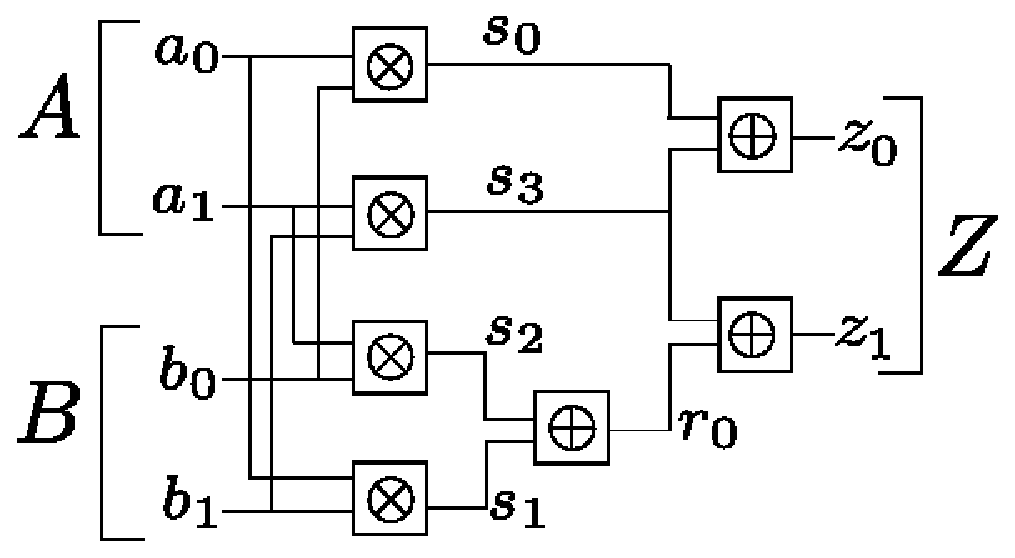
\includegraphics[scale=0.3]{2bitmult.eps}
}
\caption{\small A 2-bit Multiplier over ${\mathbb{F}}_{2^2}$. The gate
  $\otimes$ corresponds to AND-gate, i.e. bit-level multiplication
  modulo 2. The gate $\oplus$ corresponds to XOR-gate, i.e. addition
  modulo 2.} 
\label{fig:mul2bit}
\end{figure}

The functionality of the entire circuit can be described using the
following polynomials derived from the Boolean gate-level operators: 
$f_1: z_0+z_1\alpha +Z; ~~f_2: b_0+b_1\alpha +B; ~~f_3: a_0+a_1 \alpha
+A; ~~f_4: s_0+a_0 \cdot b_0; ~~f_5: s_1+a_0 \cdot b_1; ~~f_6:
s_2+a_1 \cdot b_0; ~~f_7: s_3+a_1 \cdot b_1; ~~f_8: r_0+s_1 + s_2;
~~f_9: z_0+s_0 + s_3; ~~f_{10}: z_1 + r_0 + s_3$. Ideal $J = \langle
f_1, \dots, f_{10}\rangle$. Generate $J_0$ as the ideal of vanishing
polynomials. Impose the
following {\bf elimination} term order: {\bf lex term order} with
``circuit variables'' $>$ ``Output Z'' $>$ ``Inputs, A, B''
%More precisely, we can use {\bf lex} term order with $s_0 > s_1 >  s_2 >
%s_3 >  r_0 > a_0 > a_1 > b_0 > b_1 > g_0 > g_1 > A > B > G$.
%The above term order is an {\bf elimination} order. If we use the above
and compute a Gr\"obner basis $G$ of $J + J_0$, we observe
the following polynomials in the basis:  $g_1: z_0+z_1\alpha +Z;
~~g_2: b_0+b_1\alpha +B; ~~g_3: a_0+a_1 \alpha +A; ~~g_4: s_3+r_0+z_1;
g_5: s_1+s_2+r_0; ~~g_6: s_0+s_3+z_0; ~~{\mathbf{g_7: Z +  AB}}; ~~g_8:
a_1b_1+a_1B+b_1A+z_1; ~~g_9: r_0+a_1b_1+z_1; ~~g_{10}:
s_2+a_1b_0$, and the polynomials of $J_0$. Notice that the polynomial
$g_7: Z + AB$ describes $Z = AB$ as the (canonical) polynomial
function implemented by the circuit; and we were able to {\bf extract}
this representation using the Gr\"obner basis computation. 
%We wish to explore such an approach to
%derive an efficient decision procedure for word-level abstraction. 
}
\end{Example}





